\documentclass{standalone}
\usepackage{tikz}
\usetikzlibrary{patterns, positioning}


\begin{document}
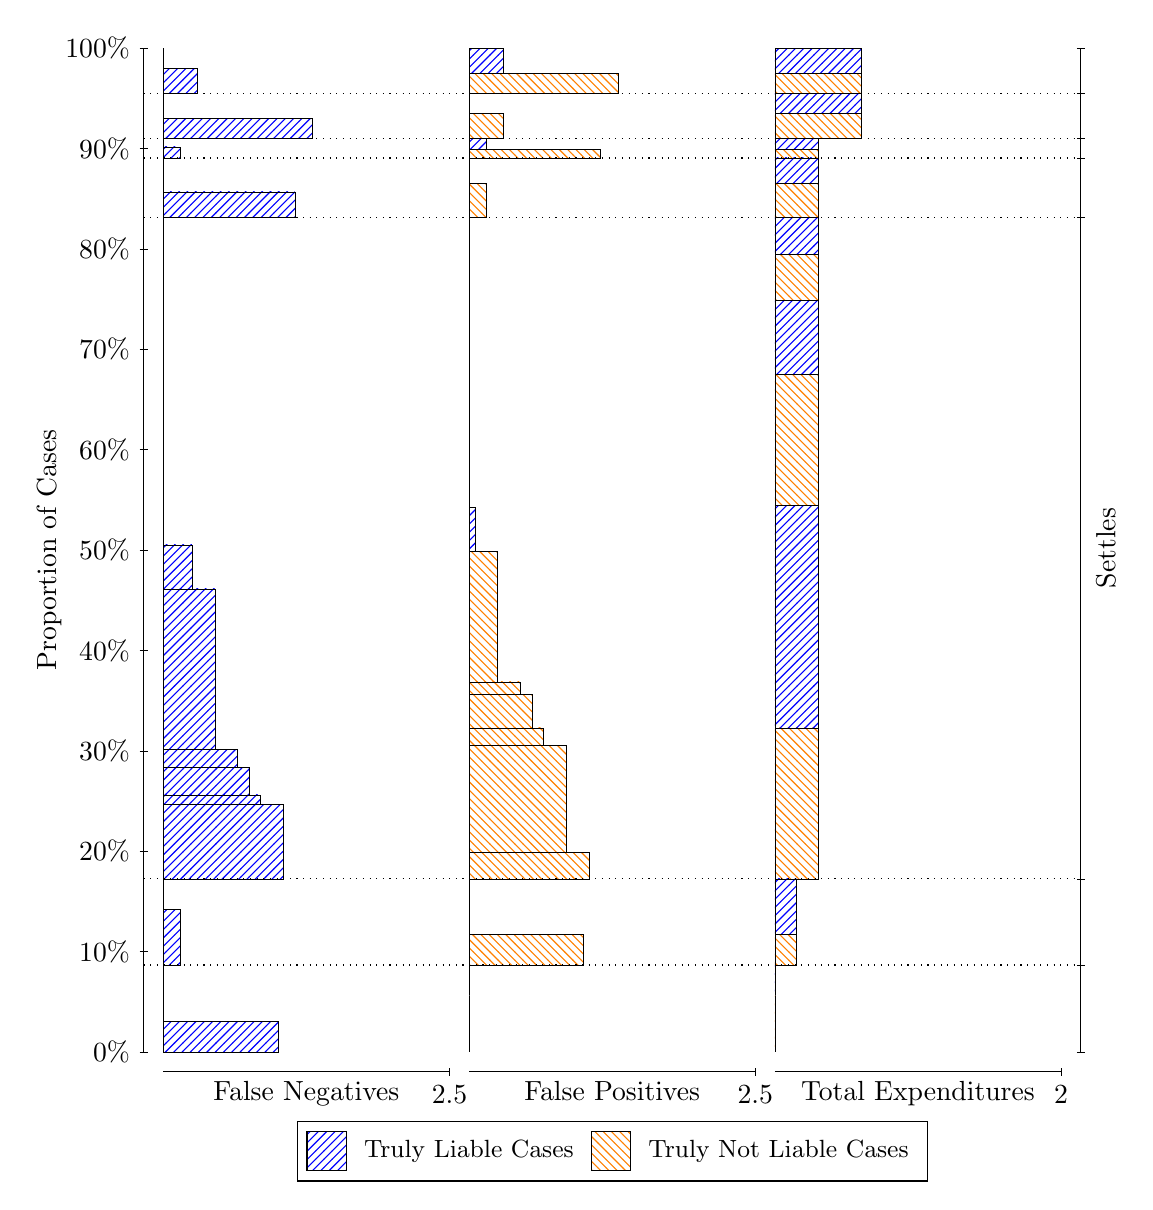
\begin{tikzpicture}
\draw[black, very thin] (1.5,1.75) -- (1.5,14.5);
\node[rotate=90, text=black, anchor=center] at (0.3, 8.125) {Proportion of Cases};
\draw[black, very thin] (1.45,1.75) -- (1.55,1.75);
\node[text=black, anchor=east] at (1.45, 1.75) {0\%};
\draw[black, very thin] (1.45,3.025) -- (1.55,3.025);
\node[text=black, anchor=east] at (1.45, 3.025) {10\%};
\draw[black, very thin] (1.45,4.3) -- (1.55,4.3);
\node[text=black, anchor=east] at (1.45, 4.3) {20\%};
\draw[black, very thin] (1.45,5.575) -- (1.55,5.575);
\node[text=black, anchor=east] at (1.45, 5.575) {30\%};
\draw[black, very thin] (1.45,6.85) -- (1.55,6.85);
\node[text=black, anchor=east] at (1.45, 6.85) {40\%};
\draw[black, very thin] (1.45,8.125) -- (1.55,8.125);
\node[text=black, anchor=east] at (1.45, 8.125) {50\%};
\draw[black, very thin] (1.45,9.4) -- (1.55,9.4);
\node[text=black, anchor=east] at (1.45, 9.4) {60\%};
\draw[black, very thin] (1.45,10.675) -- (1.55,10.675);
\node[text=black, anchor=east] at (1.45, 10.675) {70\%};
\draw[black, very thin] (1.45,11.95) -- (1.55,11.95);
\node[text=black, anchor=east] at (1.45, 11.95) {80\%};
\draw[black, very thin] (1.45,13.225) -- (1.55,13.225);
\node[text=black, anchor=east] at (1.45, 13.225) {90\%};
\draw[black, very thin] (1.45,14.5) -- (1.55,14.5);
\node[text=black, anchor=east] at (1.45, 14.5) {100\%};

\draw[black, very thin] (13.4,1.75) -- (13.4,14.5);
\draw[black, very thin] (13.35,1.75) -- (13.45,1.75);
\node[anchor=west] at (13.35, 1.75) {};
\draw[black, very thin] (13.35,2.8545) -- (13.45,2.8545);
\node[anchor=west] at (13.35, 2.8545) {};
\draw[black, very thin] (13.35,3.9491) -- (13.45,3.9491);
\node[anchor=west] at (13.35, 3.9491) {};
\draw[black, very thin] (13.35,12.352) -- (13.45,12.352);
\node[anchor=west] at (13.35, 12.352) {};
\draw[black, very thin] (13.35,13.104) -- (13.45,13.104);
\node[anchor=west] at (13.35, 13.104) {};
\draw[black, very thin] (13.35,13.35) -- (13.45,13.35);
\node[anchor=west] at (13.35, 13.35) {};
\draw[black, very thin] (13.35,13.925) -- (13.45,13.925);
\node[anchor=west] at (13.35, 13.925) {};
\draw[black, very thin] (13.35,14.5) -- (13.45,14.5);
\node[anchor=west] at (13.35, 14.5) {};

\draw[black, very thin, pattern color=blue, pattern=north east lines] (1.75,1.75) rectangle (3.2033,2.1392);
\draw[black, very thin, pattern color=orange, pattern=north west lines] (1.75,2.1392) rectangle (1.75,2.8545);
\draw[black, very thin, pattern color=blue, pattern=north east lines] (1.75,2.8545) rectangle (1.968,3.5648);
\draw[black, very thin, pattern color=orange, pattern=north west lines] (1.75,3.5648) rectangle (1.75,3.9491);
\draw[black, very thin, pattern color=blue, pattern=north east lines] (1.75,3.9491) rectangle (3.276,4.8897);
\draw[black, very thin, pattern color=blue, pattern=north east lines] (1.75,4.8897) rectangle (2.9853,5.0147);
\draw[black, very thin, pattern color=blue, pattern=north east lines] (1.75,5.0147) rectangle (2.84,5.3629);
\draw[black, very thin, pattern color=blue, pattern=north east lines] (1.75,5.3629) rectangle (2.6947,5.5899);
\draw[black, very thin, pattern color=blue, pattern=north east lines] (1.75,5.5899) rectangle (2.404,7.6318);
\draw[black, very thin, pattern color=blue, pattern=north east lines] (1.75,7.6318) rectangle (2.1133,8.1893);
\draw[black, very thin, pattern color=orange, pattern=north west lines] (1.75,8.1893) rectangle (1.75,12.352);
\draw[black, very thin, pattern color=blue, pattern=north east lines] (1.75,12.352) rectangle (3.4213,12.672);
\draw[black, very thin, pattern color=orange, pattern=north west lines] (1.75,12.672) rectangle (1.75,13.104);
\draw[black, very thin, pattern color=blue, pattern=north east lines] (1.75,13.104) rectangle (1.968,13.244);
\draw[black, very thin, pattern color=orange, pattern=north west lines] (1.75,13.244) rectangle (1.75,13.35);
\draw[black, very thin, pattern color=blue, pattern=north east lines] (1.75,13.35) rectangle (3.6393,13.606);
\draw[black, very thin, pattern color=orange, pattern=north west lines] (1.75,13.606) rectangle (1.75,13.925);
\draw[black, very thin, pattern color=blue, pattern=north east lines] (1.75,13.925) rectangle (2.186,14.244);
\draw[black, very thin, pattern color=orange, pattern=north west lines] (1.75,14.244) rectangle (1.75,14.5);
\draw[black, very thin, pattern color=orange, pattern=north west lines] (5.6333,1.75) rectangle (5.6333,2.4652);
\draw[black, very thin, pattern color=blue, pattern=north east lines] (5.6333,2.4652) rectangle (5.6333,2.8545);
\draw[black, very thin, pattern color=orange, pattern=north west lines] (5.6333,2.8545) rectangle (7.0867,3.2388);
\draw[black, very thin, pattern color=blue, pattern=north east lines] (5.6333,3.2388) rectangle (5.6333,3.9491);
\draw[black, very thin, pattern color=orange, pattern=north west lines] (5.6333,3.9491) rectangle (7.1593,4.283);
\draw[black, very thin, pattern color=orange, pattern=north west lines] (5.6333,4.283) rectangle (6.8687,5.6391);
\draw[black, very thin, pattern color=orange, pattern=north west lines] (5.6333,5.6391) rectangle (6.578,5.8661);
\draw[black, very thin, pattern color=orange, pattern=north west lines] (5.6333,5.8661) rectangle (6.4327,6.2915);
\draw[black, very thin, pattern color=orange, pattern=north west lines] (5.6333,6.2915) rectangle (6.2873,6.449);
\draw[black, very thin, pattern color=orange, pattern=north west lines] (5.6333,6.449) rectangle (5.9967,8.1122);
\draw[black, very thin, pattern color=blue, pattern=north east lines] (5.6333,8.1122) rectangle (5.706,8.6696);
\draw[black, very thin, pattern color=blue, pattern=north east lines] (5.6333,8.6696) rectangle (5.6333,12.352);
\draw[black, very thin, pattern color=orange, pattern=north west lines] (5.6333,12.352) rectangle (5.8513,12.784);
\draw[black, very thin, pattern color=blue, pattern=north east lines] (5.6333,12.784) rectangle (5.6333,13.104);
\draw[black, very thin, pattern color=orange, pattern=north west lines] (5.6333,13.104) rectangle (7.3047,13.21);
\draw[black, very thin, pattern color=blue, pattern=north east lines] (5.6333,13.21) rectangle (5.8513,13.35);
\draw[black, very thin, pattern color=orange, pattern=north west lines] (5.6333,13.35) rectangle (6.0693,13.669);
\draw[black, very thin, pattern color=blue, pattern=north east lines] (5.6333,13.669) rectangle (5.6333,13.925);
\draw[black, very thin, pattern color=orange, pattern=north west lines] (5.6333,13.925) rectangle (7.5227,14.181);
\draw[black, very thin, pattern color=blue, pattern=north east lines] (5.6333,14.181) rectangle (6.0693,14.5);
\draw[black, very thin, pattern color=orange, pattern=north west lines] (9.5167,1.75) rectangle (9.5167,2.4652);
\draw[black, very thin, pattern color=blue, pattern=north east lines] (9.5167,2.4652) rectangle (9.5167,2.8545);
\draw[black, very thin, pattern color=orange, pattern=north west lines] (9.5167,2.8545) rectangle (9.7892,3.2388);
\draw[black, very thin, pattern color=blue, pattern=north east lines] (9.5167,3.2388) rectangle (9.7892,3.9491);
\draw[black, very thin, pattern color=orange, pattern=north west lines] (9.5167,3.9491) rectangle (10.062,5.8661);
\draw[black, very thin, pattern color=blue, pattern=north east lines] (9.5167,5.8661) rectangle (10.062,8.6925);
\draw[black, very thin, pattern color=orange, pattern=north west lines] (9.5167,8.6925) rectangle (10.062,10.356);
\draw[black, very thin, pattern color=blue, pattern=north east lines] (9.5167,10.356) rectangle (10.062,11.296);
\draw[black, very thin, pattern color=orange, pattern=north west lines] (9.5167,11.296) rectangle (10.062,11.879);
\draw[black, very thin, pattern color=blue, pattern=north east lines] (9.5167,11.879) rectangle (10.062,12.352);
\draw[black, very thin, pattern color=orange, pattern=north west lines] (9.5167,12.352) rectangle (10.062,12.784);
\draw[black, very thin, pattern color=blue, pattern=north east lines] (9.5167,12.784) rectangle (10.062,13.104);
\draw[black, very thin, pattern color=orange, pattern=north west lines] (9.5167,13.104) rectangle (10.062,13.21);
\draw[black, very thin, pattern color=blue, pattern=north east lines] (9.5167,13.21) rectangle (10.062,13.35);
\draw[black, very thin, pattern color=orange, pattern=north west lines] (9.5167,13.35) rectangle (10.607,13.669);
\draw[black, very thin, pattern color=blue, pattern=north east lines] (9.5167,13.669) rectangle (10.607,13.925);
\draw[black, very thin, pattern color=orange, pattern=north west lines] (9.5167,13.925) rectangle (10.607,14.181);
\draw[black, very thin, pattern color=blue, pattern=north east lines] (9.5167,14.181) rectangle (10.607,14.5);
\draw[black, dotted] (1.5,2.8545) -- (13.4,2.8545);
\draw[black, dotted] (1.5,3.9491) -- (13.4,3.9491);
\draw[black, dotted] (1.5,12.352) -- (13.4,12.352);
\draw[black, dotted] (1.5,13.104) -- (13.4,13.104);
\draw[black, dotted] (1.5,13.35) -- (13.4,13.35);
\draw[black, dotted] (1.5,13.925) -- (13.4,13.925);
\draw[black, very thin] (1.75,1.5) -- (5.3833,1.5);
\node[text=black, anchor=north] at (3.5667, 1.5) {False Negatives};
\draw[black, very thin] (5.3833,1.45) -- (5.3833,1.55);
\node[text=black, anchor=north] at (5.3833, 1.45) {2.5};

\draw[black, very thin] (5.6333,1.5) -- (9.2667,1.5);
\node[text=black, anchor=north] at (7.45, 1.5) {False Positives};
\draw[black, very thin] (9.2667,1.45) -- (9.2667,1.55);
\node[text=black, anchor=north] at (9.2667, 1.45) {2.5};

\draw[black, very thin] (9.5167,1.5) -- (13.15,1.5);
\node[text=black, anchor=north] at (11.333, 1.5) {Total Expenditures};
\draw[black, very thin] (13.15,1.45) -- (13.15,1.55);
\node[text=black, anchor=north] at (13.15, 1.45) {2};



\node[text=black, centered, rotate=90] at (13.72, 8.1507) {Settles};





\draw (7.449999999999999,1.5) node[draw=none] (baseCoordinate) {};
\begin{scope}[align=center]
        \matrix[scale=0.5, draw=black, below=0.5cm of baseCoordinate, nodes={draw}, column sep=0.1cm]{
            \node[rectangle, draw, minimum width=0.5cm, minimum height=0.5cm, pattern color=blue, pattern=north east lines] {}; &
            \node[draw=none, font=\small, text=black] (B) {Truly Liable Cases}; &
            \node[rectangle, draw, minimum width=0.5cm, minimum height=0.5cm, pattern color=orange, pattern=north west lines] {}; &
            \node[draw=none, font=\small, text=black] (B) {Truly Not Liable Cases}; \\
            };
\end{scope}

\end{tikzpicture}
\end{document}